\documentclass[fullpage]{article}
\usepackage{graphicx}
\usepackage{enumerate}

\title{\vspace*{-2cm}\bf Assignment 2 - COMP 3400}
\author{Khalil Van Alphen\\
Student Number: 100863992\\
Email: \  khalil.va@gmail.com}
\date{}
\begin{document}
\maketitle
\pagestyle{plain}
\thispagestyle{empty}

\noindent 1. \ Prove using {\bf PROPOSITIONAL} logic and Prover9 that the map that includes Chile, Peru, Argentina and Bolivia cannot be painted with two colors if adjacent countries must have different colors. To simplify, assume that the colors are blue and green.\

\begin{enumerate}[(a)]
\item  Before doing anything with Prover9 (and independently from its input file), write the knowledge basis in propositional logic. 

\noindent {\bf Solution:} \ We will use the propositional variables as listed below:
\begin{itemize}
\item[$Pg$:]~ {\em Peru is GREEN}
\item[$Pb$:]~ {\em Peru is BLUE}
\item[$Cg$:]~ {\em Chile is GREEN}
\item[$Cb$:]~ {\em Chile is BLUE}
\item[$Bg$:]~ {\em Bolivia is GREEN}
\item[$Bb$:]~ {\em Bolivia is BLUE}
\item[$Ag$:]~ {\em Argentina is GREEN}
\item[$Ab$:]~ {\em Argentina is BLUE}
\end{itemize}
From the rules of the coloring, we are able to construct a the following propositional formulas:
\begin{itemize}
\item[$\varphi_0$:]~ ${Pg \leftrightarrow \neg Pb}$.
 Meaning: ``Peru cannot be green AND blue."
 \item[$\varphi_1$:]~ ${Bg \leftrightarrow \neg Bb}$.
 Meaning: ``Bolivia cannot be green AND blue."
 \item[$\varphi_2$:]~ ${Cg \leftrightarrow \neg Cb}$.
 Meaning: ``Chile cannot be green AND blue."
\item[$\varphi_3$:]~ ${Pg \leftrightarrow Bb}$.
 Meaning: ``Peru is green if and only if Bolivia is blue."
\item[$\varphi_4$:]~ ${Pg \leftrightarrow Cb}$.
 Meaning: ``Peru is green if and only if Chile is blue."
 \item[$\varphi_5$:]~ ${Bb \leftrightarrow Cg}$.
 Meaning: ``Bolivia is blue if and only if Chile is green."
  \item[$\varphi_6$:]~ ${Pb \leftrightarrow Bg}$.
 Meaning: ``Peru is blue if and only if Bolivia is green."
\end{itemize}

\item Our method for solving this problem will be to consider the countries on the map as vertices in a graph. Then our solution is a k-coloring solution. The graph in question has four vertices, and has five edges as shown below. These edges represent a border between the countries.The basic formula to generate the clauses was as such. We define a number of variables for the possible colors of each vertex. For each of the edges we can construct a formula that states that both vertex of the edge cannot be the same color. So for any vertex $V_i$ and $V_k$, we can say that either $V_i$ is not $color_1$ or $V_k$ is not $color_1$ (or both). Otherwise, they are both $color_1$ and our system is a contradiction. Example of such a clause:
${\neg (V_i is color_1) \vee \neg (V_k is color_1)}$\\

We create these for every edge (not all will be necessary for a proof). In this specific example, we can use a simpler form, as there is only two colors. In this case, we can say that not being a color is equivalent to being the other color, as all vertices must have a color. This allows us to make the assumptions in $a)$. Basically, we use the negation property as defined below:
\begin{itemize}
\item[] ${\neg Pg = Pb}$
\item[] ${\neg Cg = Cb}$
\item[] ${\neg Bg = Bb}$
\item[] ${\neg Ag = Ab}$
\end{itemize}

We acknowledge that the method used here would not be easily translated to higher orders of color. However, the solution explained above would be very easily applied to any number of colors.
\begin{figure}[h!]
\centering
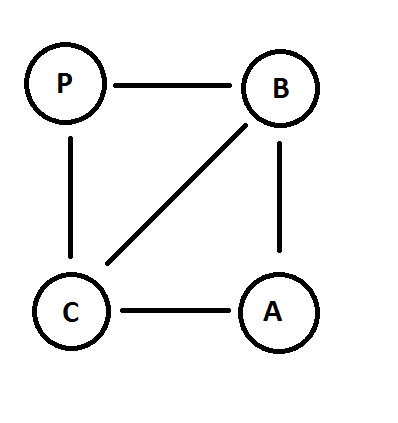
\includegraphics[scale=0.4]{graph}
\caption{Graph representation}
\label{fig:method}
\end{figure}

\item

The main section of the attached input file is as follows:

{\small
\begin{verbatim}
	formulas(assumptions).
	
	Pg.
	Pg <-> -Pb.
	Cg <-> -Cb.
	Bg <-> -Bb.

	Pg <-> Bb.
	Pg <-> Cb.
	Bb <-> Cg.
	Pb <-> Bg.

	end_of_list.

	formulas(goals).
	
	Pg.
	
	end_of_list.

 \end{verbatim}
}
 The main section of the attached output file is as follows:

 {\footnotesize \begin{verbatim}
	% Proof 1 at 0.01 (+ 0.03) seconds.
% Length of proof is 14.
% Level of proof is 4.
% Maximum clause weight is 2.
% Given clauses 0.

2 Cg <-> -Cb # label(non_clause).  [assumption].
4 Pg <-> Bb # label(non_clause).  [assumption].
5 Pg <-> Cb # label(non_clause).  [assumption].
6 Bb <-> Cg # label(non_clause).  [assumption].
8 Pg # label(non_clause) # label(goal).  [goal].
12 Cg | Cb.  [clausify(2)].
16 Pg | -Bb.  [clausify(4)].
18 Pg | -Cb.  [clausify(5)].
20 Bb | -Cg.  [clausify(6)].
23 -Pg.  [deny(8)].
24 -Cb.  [back_unit_del(18),unit_del(a,23)].
25 -Bb.  [back_unit_del(16),unit_del(a,23)].
27 Cg.  [back_unit_del(12),unit_del(b,24)].
28 $F.  [back_unit_del(20),unit_del(a,25),unit_del(b,27)].
.
\end{verbatim} }
\noindent
2. \ Do the same as in the previous problem, and with the same requests, with {\bf PREDICATE} logic. For that you can use predicates for ``being neighbors" and ``having a color", 
and symbolic constants for the four countries and the two colors.\\

\noindent {\bf Solution:} \ We will use the predicates as listed below:
\begin{itemize}
\item[$P$:]~ {\em Peru}
\item[$B$:]~ {\em Bolivia}
\item[$C$:]~ {\em Chile}
\item[$A$:]~ {\em Argentina}
\item[$b$:]~ {\em color blue}
\item[$g$:]~ {\em color green}
\item[$N(x,y)$:]~ {\em x and y share a border}
\item[$M(i,j)$:]~ {\em i has color j}
\end{itemize}
In this take on the problem we can define the following propositions:
\begin{itemize}
\item[$\varphi_0$:]~ ${N(P, B)}$.
\item[$\varphi_1$:]~ ${N(P, C)}$.
\item[$\varphi_2$:]~ ${N(B, C)}$.
\item[$\varphi_3$:]~ ${N(B, A)}$.
\item[$\varphi_4$:]~ ${N(C, A)}$.
\item[$\varphi_5$:]~ $\forall x \forall y{N(x, y) \rightarrow (\neg M(x, b) \vee \neg M(y, b)) \wedge (\neg M(x, g) \vee \neg M(y, g))}$.

Meaning: Same as above, for all of the countries, if they share a border, then that means their colors cannot be both green and cannot be both blue.
\end{itemize}

Now it is a simple matter of proving that there exists no configuration of colors for the countries that obeys these rules. We will find that the expression ${M(P, g)}$ and ${M(P, b)}$ both provide us with contradictions. See attached input/output.
\end{enumerate}

\newpage
\section*{Appendix: Input/Output Files}
1.INPUT:

 {\footnotesize \begin{verbatim}
if(Prover9). % Options for Prover9
  assign(max_seconds, 60).
end_if.

if(Mace4).   % Options for Mace4
  assign(max_seconds, 60).
end_if.

formulas(assumptions).

Pg <-> -Pb.
Cg <-> -Cb.
Bg <-> -Bb.

Pg <-> Bb.
Pg <-> Cb.
Bb <-> Cg.
Pb <-> Bg.

end_of_list.

formulas(goals).

Pg.

end_of_list.

\end{verbatim} }

1.OUTPUT:

 {\footnotesize \begin{verbatim}
============================== prooftrans ============================
Prover9 (32) version Dec-2007, Dec 2007.
Process 178728 was started by Khalil on Khalil-PC,
Thu Feb 16 19:43:22 2017
The command was "/cygdrive/c/Program Files (x86)/Prover9-Mace4/bin-win32/prover9".
============================== end of head ===========================

============================== end of input ==========================

============================== PROOF =================================

% -------- Comments from original proof --------
% Proof 1 at 0.00 (+ 0.01) seconds.
% Length of proof is 14.
% Level of proof is 4.
% Maximum clause weight is 2.
% Given clauses 0.

2 Cg <-> -Cb # label(non_clause).  [assumption].
4 Pg <-> Bb # label(non_clause).  [assumption].
5 Pg <-> Cb # label(non_clause).  [assumption].
6 Bb <-> Cg # label(non_clause).  [assumption].
8 Pg # label(non_clause) # label(goal).  [goal].
12 Cg | Cb.  [clausify(2)].
16 Pg | -Bb.  [clausify(4)].
18 Pg | -Cb.  [clausify(5)].
20 Bb | -Cg.  [clausify(6)].
23 -Pg.  [deny(8)].
24 -Cb.  [back_unit_del(18),unit_del(a,23)].
25 -Bb.  [back_unit_del(16),unit_del(a,23)].
27 Cg.  [back_unit_del(12),unit_del(b,24)].
28 $F.  [back_unit_del(20),unit_del(a,25),unit_del(b,27)].

============================== end of proof ==========================

\end{verbatim} }

2. SOURCE

{\footnotesize \begin{verbatim}
	============================== Prover9 ===============================
Prover9 (32) version Dec-2007, Dec 2007.
Process 177544 was started by Khalil on Khalil-PC,
Thu Feb 16 19:53:57 2017
The command was "/cygdrive/c/Program Files (x86)/Prover9-Mace4/bin-win32/prover9".
============================== end of head ===========================

============================== INPUT =================================
assign(report_stderr,2).
set(ignore_option_dependencies).
if(Prover9).
% Conditional input included.
assign(max_seconds,60).
end_if.
if(Mace4).
% Conditional input omitted.
end_if.

formulas(assumptions).
N(P,B).
N(P,C).
N(B,C).
N(B,A).
N(C,A).
(all x all y N(x,y)) -> -M(x,b) | -M(y,b).
(all x all y N(x,y)) -> -M(x,g) | -M(y,g).
end_of_list.

formulas(goals).
M(P,g).
end_of_list.

============================== end of input ==========================

% Enabling option dependencies (ignore applies only on input).

============================== PROCESS NON-CLAUSAL FORMULAS ==========

% Formulas that are not ordinary clauses:
1 (all x all y N(x,y)) -> -M(x,b) | -M(y,b) # label(non_clause).  [assumption].
2 (all x all y N(x,y)) -> -M(x,g) | -M(y,g) # label(non_clause).  [assumption].
3 M(P,g) # label(non_clause) # label(goal).  [goal].

============================== end of process non-clausal formulas ===

============================== PROCESS INITIAL CLAUSES ===============

% Clauses before input processing:

formulas(usable).
end_of_list.

formulas(sos).
N(P,B).  [assumption].
N(P,C).  [assumption].
N(B,C).  [assumption].
N(B,A).  [assumption].
N(C,A).  [assumption].
-N(f1(x,y),f2(x,y)) | -M(x,b) | -M(y,b).  [clausify(1)].
-N(f3(x,y),f4(x,y)) | -M(x,g) | -M(y,g).  [clausify(2)].
-M(P,g).  [deny(3)].
end_of_list.

formulas(demodulators).
end_of_list.

============================== PREDICATE ELIMINATION =================

Eliminating N/2
4 -N(f1(x,y),f2(x,y)) | -M(x,b) | -M(y,b).  [clausify(1)].
5 N(P,B).  [assumption].
6 N(P,C).  [assumption].
7 N(B,C).  [assumption].
8 N(B,A).  [assumption].
9 N(C,A).  [assumption].
10 -N(f3(x,y),f4(x,y)) | -M(x,g) | -M(y,g).  [clausify(2)].

Eliminating M/2

============================== end predicate elimination =============

Auto_denials:  (no changes).

Term ordering decisions:
Predicate symbol precedence:  predicate_order([ ]).
Function symbol precedence:  function_order([ ]).
After inverse_order:  (no changes).
Unfolding symbols: (none).

Auto_inference settings:
  % set(neg_binary_resolution).  % (HNE depth_diff=0)
  % clear(ordered_res).  % (HNE depth_diff=0)
  % set(ur_resolution).  % (HNE depth_diff=0)
    % set(ur_resolution) -> set(pos_ur_resolution).
    % set(ur_resolution) -> set(neg_ur_resolution).

Auto_process settings:  (no changes).

============================== end of process initial clauses ========

============================== CLAUSES FOR SEARCH ====================

% Clauses after input processing:

formulas(usable).
end_of_list.

formulas(sos).
end_of_list.

formulas(demodulators).
end_of_list.

============================== end of clauses for search =============

============================== SEARCH ================================

% Starting search at 0.01 seconds.

============================== STATISTICS ============================

Given=0. Generated=0. Kept=0. proofs=0.
Usable=0. Sos=0. Demods=0. Limbo=0, Disabled=8. Hints=0.
Weight_deleted=0. Literals_deleted=0.
Forward_subsumed=0. Back_subsumed=0.
Sos_limit_deleted=0. Sos_displaced=0. Sos_removed=0.
New_demodulators=0 (0 lex), Back_demodulated=0. Back_unit_deleted=0.
Demod_attempts=0. Demod_rewrites=0.
Res_instance_prunes=0. Para_instance_prunes=0. Basic_paramod_prunes=0.
Nonunit_fsub_feature_tests=0. Nonunit_bsub_feature_tests=0.
Megabytes=0.01.
User_CPU=0.01, System_CPU=0.00, Wall_clock=0.

============================== end of statistics =====================

============================== end of search =========================

SEARCH FAILED

Exiting with failure.

\end{verbatim} }

\end{document} 
